\documentclass{report}
\usepackage{graphicx} % Required for inserting images
\usepackage{geometry}
\usepackage{amsmath}
\usepackage{mathtools}
\usepackage{amssymb}
\usepackage{kotex}
\usepackage{makecell}
\usepackage{bytefield}
\usepackage{listings}
\usepackage{caption}
\usepackage{subcaption}

\captionsetup{labelformat=empty,labelsep=none,font=small}
\lstset{
    basicstyle=\small\ttfamily,
    commentstyle=\small\ttfamily,
    numbers=left,
    columns=flexible,
    breaklines=true,
    captionpos=b,
    xleftmargin=5.0ex,
    aboveskip=1.0em,
}

\title{CSED551 PA\#3 \\[0.5ex] {\normalsize :Panorama Image Generation}}
\author{\small{20220848 Minsu Sun}}
\date{\small{November 17, 2024}}

\begin{document}

\maketitle

\section*{Code}

아래는 Panorama Image Generation을 위해 작성한 함수들에 대한 설명이다.

\begin{lstlisting}[language=Python, caption=panorama, firstnumber=117]
def panorama(
    image_list: list["np.ndarray[np.uint8 | np.float32]"],
) -> "np.ndarray[np.uint8 | np.float32]":
    # 1. Given N input images, set one image as a reference
    reference_image = image_list[0]

    for source_image in image_list[1:]:
        # 2. Detect feature points from images and correspondeces between pairs of images
        kp_ref, des_ref = SIFT.detectAndCompute(reference_image, None)
        kp_src, des_src = SIFT.detectAndCompute(source_image, None)

        matches = BF.knnMatch(des_ref, des_src, k=2)

        good_matches = []
        for m, n in matches:
            if m.distance < 0.75 * n.distance:
                good_matches.append([m])

        # 3. Estimate the homographics between images using RANSAC
        H = RANSAC(good_matches, kp_ref, kp_src, reference_image, source_image)

        # 4. Warp the images to the reference image
        # 5. Compose them
        reference_image = stitch_images(reference_image, source_image, H)

    return reference_image
\end{lstlisting}

위 코드는 주어진 이미지 리스트를 이용하여 Panorama Image Generation을 진행한다.
첫 Reference 이미지는 이미지 중 첫 이미지를 선택한다.
이후 Reference 이미지 이외 나머지 이미지에 대하여 Reference 이미지와의 상관 관계를 계산한다.
SIFT(Scale Invariant Feature Transform)를 이용하여 Reference와 현재 이미지의 Feature를 추출한다.
각 Feature의 Matching은 OpenCV에서 제공하는 BFMatcher(Brute Force Matcher)의 \code{knnMatch}를 사용하였고, 이 때 설정한 \code{k}는 2이다.
\code{knnMatch}에 의해 Matching된 각 포인트들은 \code{0.75}의 Ratio Test를 통해 일부만을 사용한다.
이후 \code{RANSAC}을 이용하여 Homography \code{H}를 예측하고, 이와 \code{stitch_images}를 이용하여 이미지를 합성한다.

\begin{lstlisting}[language=Python, caption=RANSAC, firstnumber=16]
def RANSAC(matches, kp1, kp2, image1, image2) -> None:
    RANSAC_CONFIG = config._RANSAC_CONFIG()

    # Convert matches to kp pair
    matches_kp = [[kp1[match[0].queryIdx], kp2[match[0].trainIdx]] for match in matches]

    target_inlier_count = 0  # maximum inlier count
    target_inlier_pair = []

    for _ in range(RANSAC_CONFIG.N_ITERATION):
        # select random 4 pair of matching point candidates
        random_sample_idx = [random.randint(0, len(matches_kp) - 1) for _ in range(4)]

        src_p = np.asarray(
            [matches_kp[idx][0].pt for idx in random_sample_idx], np.float32
        )
        dst_p = np.asarray(
            [matches_kp[idx][1].pt for idx in random_sample_idx], np.float32
        )

        H = cv2.getPerspectiveTransform(src_p, dst_p)

        inlier = util.find_inlier(H, matches_kp, RANSAC_CONFIG.INLIER_THRESHOLD)
        inlier_count = len(inlier)
        if target_inlier_count < inlier_count:
            target_inlier_count = inlier_count
            target_inlier_pair = inlier

    src = np.asarray([[*p, 1] for p, _ in target_inlier_pair])
    dst = np.asarray([[*p, 1] for _, p in target_inlier_pair])

    # find homography
    # use least square method by specifing method = 0
    # (src: https://docs.opencv.org/4.1.0/d9/d0c/group__calib3d.html#ga4abc2ece9fab9398f2e560d53c8c9780)
    # they use LMSolver to find solution for least square problem
    hom, _ = cv2.findHomography(src, dst, 0)

    return hom
\end{lstlisting}

위 코드는 주어진 Feature Matching을 이용하여 이미지 간의 Homography를 예측하는 RANSAC 알고리즘을 구현한 것이다.
Feature Matching된 match들을 key-point pair로 변환하여 이후 Homography 예측할 수 있도록 준비한다.
4 쌍의 랜덤 페어를 찾아 각 페어별로 inling 하는 포인트 쌍의 개수를 이용해 가장 많은 inlier를 갖는 homography를 찾는다.
찾은 Homography에 의해 inling하는 페어들 전체를 대상으로 Homography를 계산한다.
이때, \code{cv2.findHomography}를 사용였는데, least square method를 사용하도록 설정하였다.
(OpenCV는 내부적으로 least square method를 지원하기 위해 Levenberg-Marquardt Solver, \code{LMSolver}를 사용한다.
해당 방법은 Gradient Descent와 Gauss-Newton 방법을 하이브리드로 사용하는 알고리즘이다.)

\begin{lstlisting}[language=Python, caption=stitch\_images, firstnumber=56]
def stitch_images(
    ref: "np.array[np.uint8 | np.float32]",
    src: "np.array[np.uint8 | np.float32]",
    H: "np.array[np.uint8]",
) -> "np.array[np.float32]":
    ref_height, ref_width, _ = ref.shape
    src_height, src_width, _ = src.shape

    H_Inv = np.linalg.inv(H)

    x1, y1 = util.transform(0, 0, H_Inv)
    x2, y2 = util.transform(0, src_height - 1, H_Inv)
    x3, y3 = util.transform(src_width - 1, 0, H_Inv)
    x4, y4 = util.transform(src_width - 1, src_height - 1, H_Inv)

    min_x = np.round(min(0, x1, x2, x3, x4)).astype(int)
    min_y = np.round(min(0, y1, y2, y3, y4)).astype(int)
    max_x = np.round(max(ref_width, x1, x2, x3, x4)).astype(int)
    max_y = np.round(max(ref_height, y1, y2, y3, y4)).astype(int)

    ofs_x = np.abs(min_x)
    ofs_y = np.abs(min_y)

    height = ofs_y + ref_height + np.abs(ref_height - max_y)
    width = ofs_x + ref_width + np.abs(ref_width - max_x)

    image = np.zeros((height, width, 3))

    # Paste reference image
    image[ofs_y : ofs_y + ref_height, ofs_x : ofs_x + ref_width, :] = ref

    # Generate distance transformation for alpha blending
    # Alpha for blending will be determined by this
    mask = np.zeros((src_width + 2, src_height + 2), np.uint8)
    mask[1 : 1 + src_width, 1 : 1 + src_height] = np.ones((src_width, src_height)) * 255
    _, t = cv2.threshold(mask, 0, 255, cv2.THRESH_BINARY + cv2.THRESH_OTSU)
    mask = cv2.distanceTransform(t, cv2.DIST_L2, 5) / 255

    for y in range(min_y, height):
        for x in range(min_x, width):
            if y + ofs_y < height and x + ofs_x < width:
                # Warp the position of pixel
                xp, yp = util.transform(x, y, H)

                if 0 < xp < src_width and 0 < yp < src_height:
                    # Retrieve full pixel
                    pixel = cv2.getRectSubPix(src, (1, 1), (xp, yp))

                    # For non-empty pixels, conduct alpha blending
                    if not np.all(image[y + ofs_y, x + ofs_x] == 0):
                        r = mask[int(xp), int(yp)]
                        image[y + ofs_y, x + ofs_x] = pixel * r + image[
                            y + ofs_y, x + ofs_x
                        ] * (1 - r)
                    # For empty pixels, copy warped pixel
                    else:
                        image[y + ofs_y, x + ofs_x] = pixel

    return image.astype(np.uint8)
\end{lstlisting}

위 코드는 RANSAC에 의하여 계산된 Homography를 이용해 Source 이미지를 Reference 이미지에 Stitch하는 함수를 구현한 것이다.
주어진 Homography의 Inverse를 계산해 Source 이미지의 각 꼭지점이 Warp되었을 때의 위치를 계산한 후, Stitch된 이미지의 너비와 높이를 결정한다.
결정된 높이와 너비를 이용하여 빈 이미지를 만들고 기존 Reference 이미지를 그대로 붙인다.
이후 Source 이미지에 대해 Distance Transformation을 진행한다.
이는 이후 Seaming을 제거하기 위한 것으로, Source 이미지의 크기대로 block image를 만들어 계산하였다.
이미지 공간에서 Source 이미지로부터 Warp될 위치마다 Source 이미지의 픽셀을 가져와 합성한다.
Reference 이미지에 의하여 이미 채워진 공간이라면, 위에서 계산한 Distance Transformation을 이용해 Alpha Blending을 진행한다.
이 때, Distance Transformation은 테두리로 접근할 수록 weight가 낮아지는 형태를 가지기에 seaming을 제거하는데 탁월하다.
작업 완료 후 결과 이미지를 반환한다.

\newpage

\section*{Details and Configuration}

아래는 주요 연산에서 사용되었던 세부 계산 함수들이다.

\begin{lstlisting}[language=Python, caption=util.py, firstnumber=1]
import numpy as np


def transform(x, y, H):
    h = np.array([x, y, 1])
    t = H.dot(h)
    w = t[2]
    return t[0] / w, t[1] / w


def match_distance(match, H):
    x, y = transform(*match[0].pt, H)
    return np.sqrt((x - match[1].pt[0]) ** 2 + (y - match[1].pt[1]) ** 2)


def find_inlier(H, matches, threshold):
    inlier = [
        [match[0].pt, match[1].pt]
        for match in matches
        if match_distance(match, H) < threshold
    ]
    return inlier
\end{lstlisting}

\begin{itemize}
    \item \code{transform}: 주어진 Homography \code{H}를 이용하여 Homogenous Coordinate에서의 Transformation 이후 다시 Cartesian Coordinate로 변환하여 반환한다.
    \item \code{match_distance}: match의 각 key point가 주어진 Homography \code{H} 기준으로의 거리를 계산한다.
    \item \code{find_inlier}: 주어진 match 중에서 \code{threshold} 이하의 match인 inlier를 찾아 리스트로 반환한다.
\end{itemize}

다음은 RANSAC 알고리즘에서 사용된 설정이다.

\begin{lstlisting}[language=Python, caption=config.py, firstnumber=1]
class _RANSAC_CONFIG:
    N_ITERATION = 100
    INLIER_THRESHOLD = 5
\end{lstlisting}

\newpage

\section*{Visualization}

\subsection*{Input Images}

다음은 과제 진행에 사용된 이미지들이다.

\begin{figure}[htbp]
    \centering

    \subfloat[Rainier1.png]{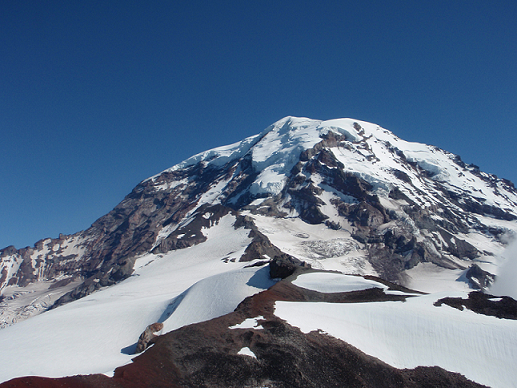
\includegraphics[width=0.17\linewidth]{../images/input/Rainier1.png}}
    \hspace{1pt}
    \subfloat[Rainier2.png]{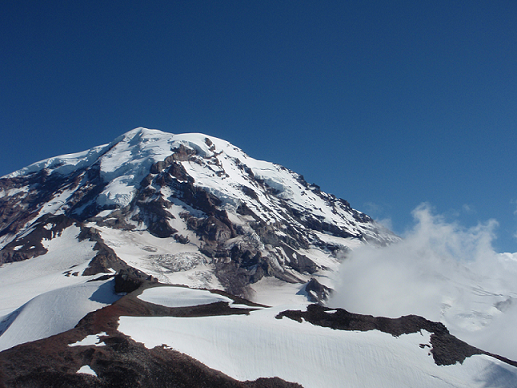
\includegraphics[width=0.17\linewidth]{../images/input/Rainier2.png}}
    \hspace{1pt}
    \subfloat[Rainier3.png]{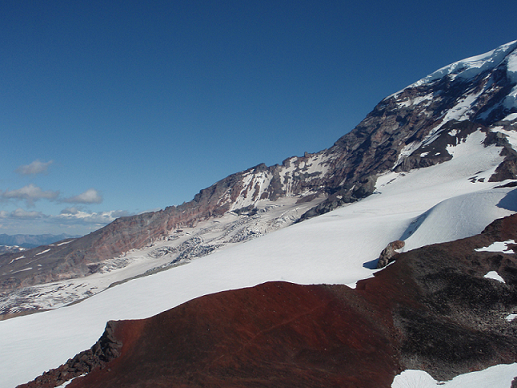
\includegraphics[width=0.17\linewidth]{../images/input/Rainier3.png}}
    \hspace{1pt}
    \subfloat[Rainier4.png]{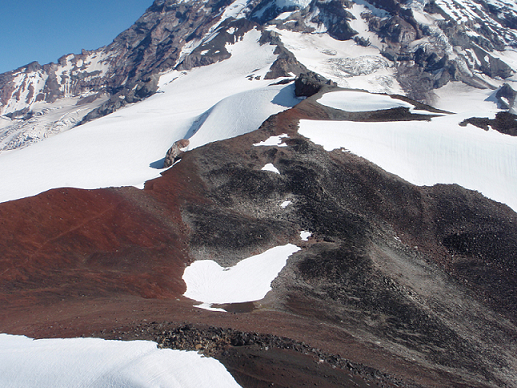
\includegraphics[width=0.17\linewidth]{../images/input/Rainier4.png}}
    \hspace{1pt}
    \subfloat[Rainier5.png]{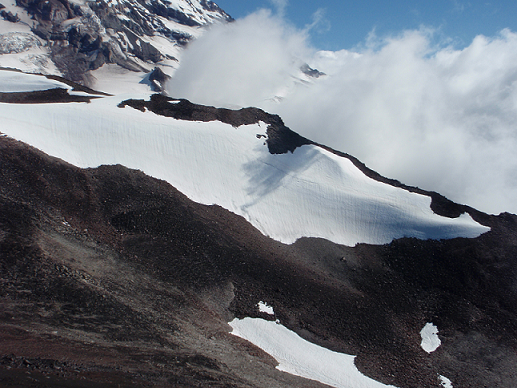
\includegraphics[width=0.17\linewidth]{../images/input/Rainier5.png}}

    \caption{Input Images}
\end{figure}

\subsection*{Output Image}

위의 Input Images를 이용하여 Panorama Image Generation을 완료된 결과는 아래의 이미지와 같다.

\begin{figure}[htbp]
    \centering

    \subfloat[stitched.png]{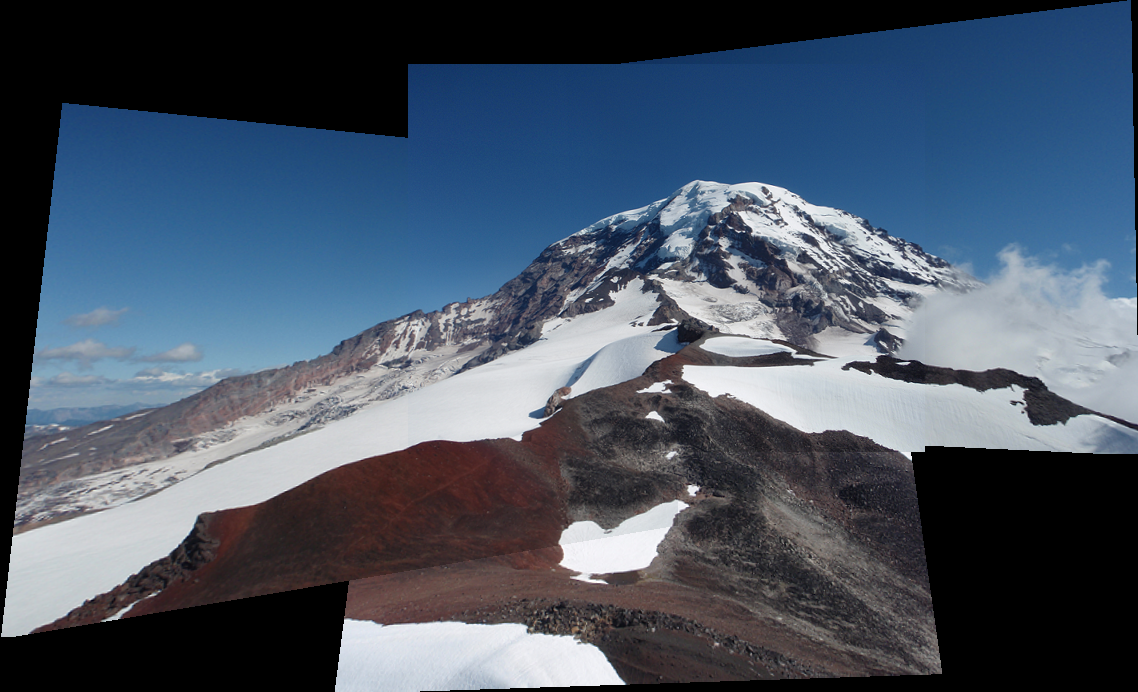
\includegraphics[width=0.45\linewidth]{../images/output/stitched.png}}

    \caption{Input Images}
\end{figure}

Distance Transformatoin을 이용하여 Alpha Blending을 적용한 의도에 부합하도록 결과 이미지가 생성된 것을 확인할 수 있다.

\newpage

\section*{Discussion}

사용한 이미지 이외에 아래와 같은 추가 이미지를 이용하여 다시 Generation을 하는 경우 그 아래와 같이 이전에는 없는 seaming을 관찰할 수 있다.
(왼쪽 하단 하늘 부분)
이는 새로 추가한 이미지의 대비, 밝기, 채도 등이 기존에 사용하였던 이미지와 큰 차이가 남에 따라 Alpha Blending을 진행하여도 발생하는 결과로 생각된다.
이에 대한 해결책으로는 사용되는 이미지들의 대비, 밝기, 채도 등을 최대한 비슷하게 사용하는 것을 제시할 수 있다.
해당하는 방법으로는 Histogram Equalization이나 Gamma Correction 등이 있다.

\begin{figure}[htbp]
    \centering

    \subfloat[New image - images/input/addition.png]{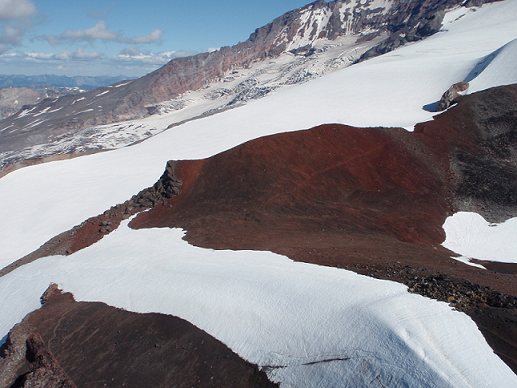
\includegraphics[width=0.4\linewidth]{../images/input/addition.png}}
    \hspace{1pt}
    \subfloat[Abnormal Result - images/output/abnormal.png]{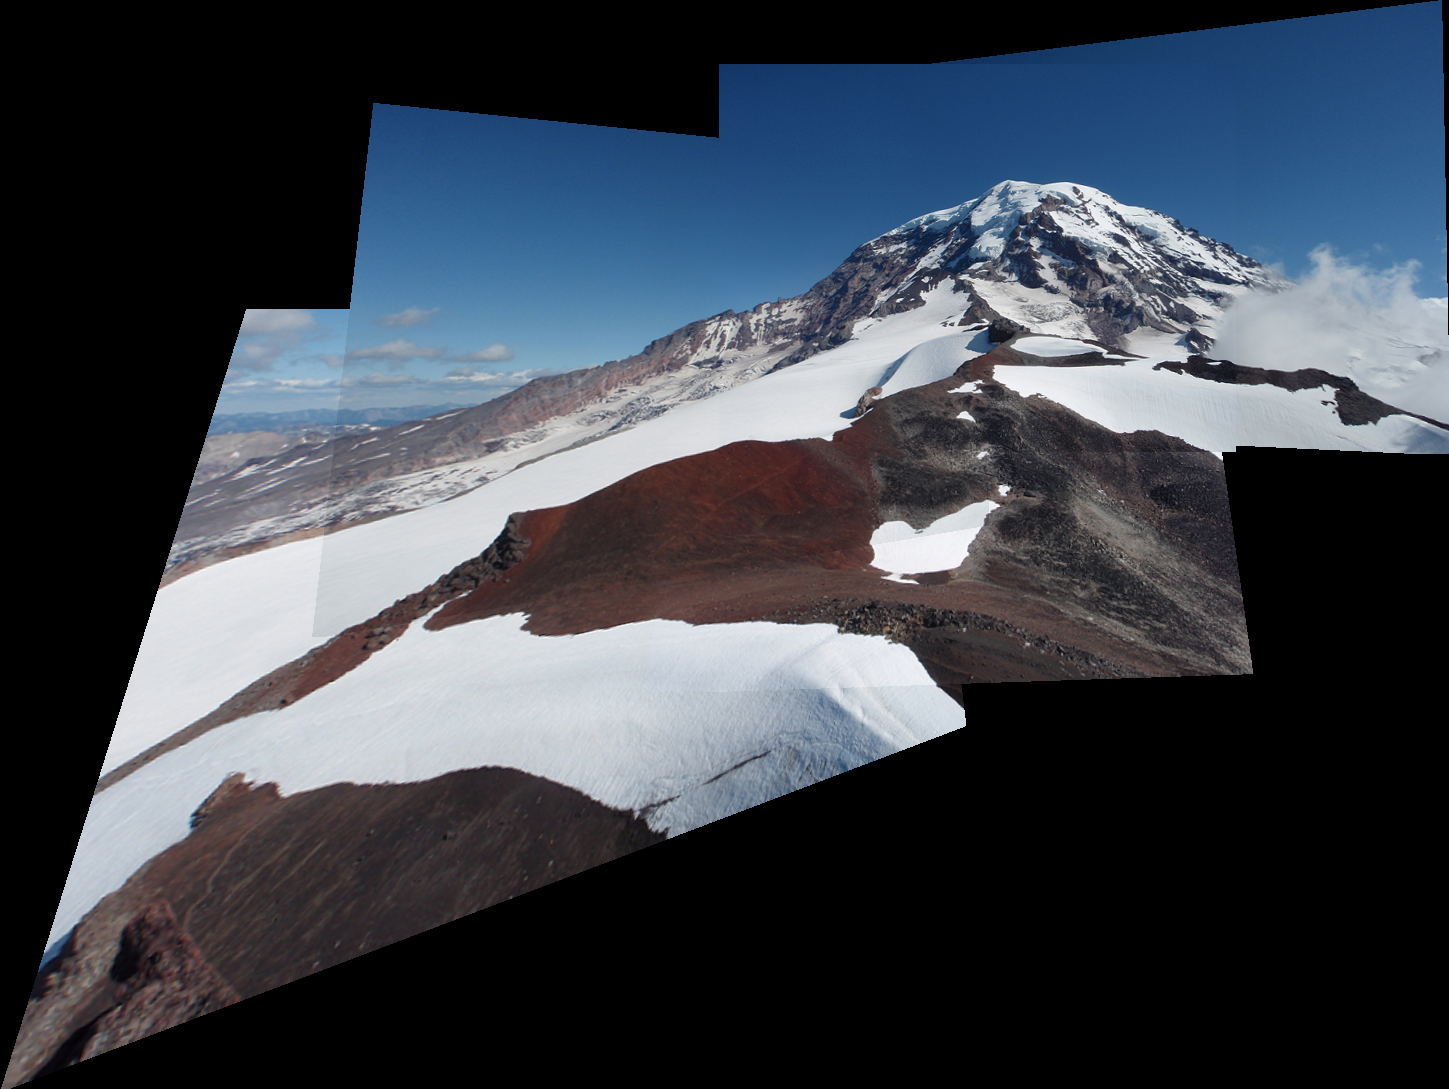
\includegraphics[width=0.4\linewidth]{../images/output/abnormal.png}}

    \caption{Discussion}
\end{figure}

\end{document}
